\documentclass[12pt]{article}

\usepackage[utf8]{inputenc}
\usepackage[T1]{fontenc}
\usepackage{geometry}
\usepackage{graphicx} %figures
\usepackage{subfig} %subfigures
\usepackage{gensymb} %degree sign
\usepackage{amsmath} %math stuff
\usepackage{bm} %bold stuff
\usepackage[]{algorithm2e} %algorithms
\geometry{a4paper}

\title{\textbf{Part 8: Breaking Down BOtorch}}

\begin{document}
\date{January 25, 2021}
\maketitle

Hello and welcome to the 8th post! Today will be a short one. We'll be talking about BOtorch (Bayesian optimization within a python framework) that will hopefully let us explore some more complex models rather than writing them all out by hand.

\vspace{5mm}

First off we will plot the original toy problem $f(x)=x_1^2+x_2^2$. For the first GP approximation we will use a simple noise free model. For a more complex example we will design our own acquisition function $\alpha(x)$. BOtorch provides us with many nice ways of optimizing things, but to understand how to use these tools it is best to break down what they do. We will use a simple $\alpha(x)=f(x)$, or the posterior approximation of the GP mean is the acquisition function (see Figure 1c).

\vspace{5mm}

Using the same philosophy as designing our own acquisition function, we will design our own optimizer. Of course using $\alpha(x)$ we can build any number of zeroth order optimizer (genetic algorithms for example) but BOtorch gives us a means to optimize using the open source python package sklearn. I will use the most generic method they have and run multi-start optimization over the above model. The solution to the optimization problem is in red.

\begin{figure}[h]
\centering
\subfloat[][Real $f(x)$]{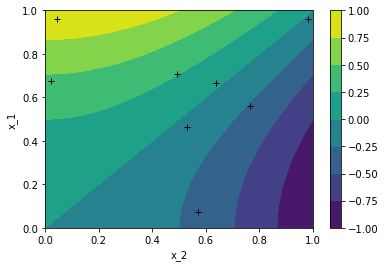
\includegraphics[width=0.35\textwidth]{Post_8_fig1}}
\subfloat[][GP Approx. 1]{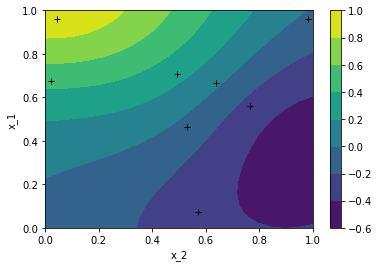
\includegraphics[width=0.35\textwidth]{Post_8_fig2}}
\subfloat[][GP Approx. 2]{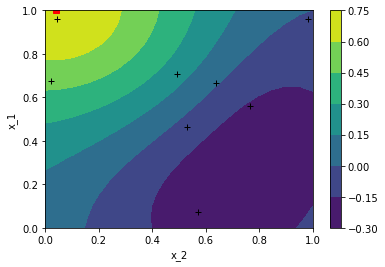
\includegraphics[width=0.35\textwidth]{Post_8_fig3}}
\caption{Toy Problem}
\end{figure}

\vspace{5mm}

While this is a short post today, working with other people's code is much harder than writing our own. It took me far less time to write my own GPs that are just as powerful as those in BOtorch, however it is also useful to understand other methods to (i) better our own implementations (ii) be able to solve hard problems with the tools at hand and (iii) a third reason.

\vspace{5mm}

It was not too much fun to do this so next week we are going to go over Stochastic Gradient Descent as a treat!

\end{document}